\section{User Guide}
This section contains information directed specifically to users. It contains clear descriptions of what inputs are needed and what effect they have. It should also help the user be able to use the model for the first time. Some possible examples are included below:

\subsection{Variable Definition and Code Description}
The variables in Table \ref{tabular:vars} are available for user input. Variables used by the module but not available to the user are not mentioned here. Variables with default settings do not necessarily need to be changed by the user, but may be.
\begin{table}[H]
	\caption{Definition and Explanation of Variables Used.}
	\label{tab:errortol}
	\centering \fontsize{10}{10}\selectfont
	\begin{tabular}{ | m{5cm}| m{2cm} | m{1.5cm} | m{6cm} |} % Column formatting, 
		\hline
		\textbf{Variable}   		& \textbf{LaTeX Equivalent} 	                  &		\textbf{Variable Type}   & \textbf{Notes} \\ \hline
		stateInMsgName			&N/A		   							    & string 								& Default setting: ``inertial\_state\_output". This is the message from which the radiation pressure module receives spacecraft inertial data.\\ \hline
		sunEphmInMsgName	& N/A 										& string 								& Default setting: ``sun\_planet\_data". This is the message through which radiation pressure gets information about the sun and planets.\\ \hline
		area 						  	  & $A_{\odot}$							  & double 								& [m2] Default setting: 0.0f. Required input for cannonball method to get any real output. This is the area to use when approximating the surface area of the spacecraft.\\ \hline
		coefficientReflection 	  & $c_{R}$ 								& double 								& Default setting: 1.2. This is a factor applied to the radiation pressure based on spacecraft surface properties.\\ \hline
		useCannonballModel	   & N/A 									   & bool 									& Default setting: True. To switch cannonball mode off, use the call setUseCanonballModel(``False")\\ \hline
		sunEclipseInMsgName	 & N/A 										 & string									& No default. Must be set. If an eclipse model is being used, this should reference eclipse output. \\ \hline
		sunEclipseMsgData		& N/A										& string									& No default. If creating a "fake" eclipse message, set to radiation\_pressure.EclipseSimMsg() \\ \hline
		sunEclipseMsgData.shadowFactor & $F_{\mathrm{s}}$& double								& Default setting: 1.0. i.e. there is no shadow by default. \\ \hline
	\end{tabular}
	\label{tabular:vars}
\end{table}

It is important to note that in order for the sunEclipse information in the table above to be utilized, one must call:
unitTestSupport.setMessage(unitTestSim.TotalSim, testProcessName, sunEclipseInMsgName, sunEclipseMsgData). In other cases, the eclipse message will be set by the eclipse module and the radiation pressure module will only need to be told where to look for it.

\subsubsection{Code Diagram}

\begin{figure}[H]
	\centering 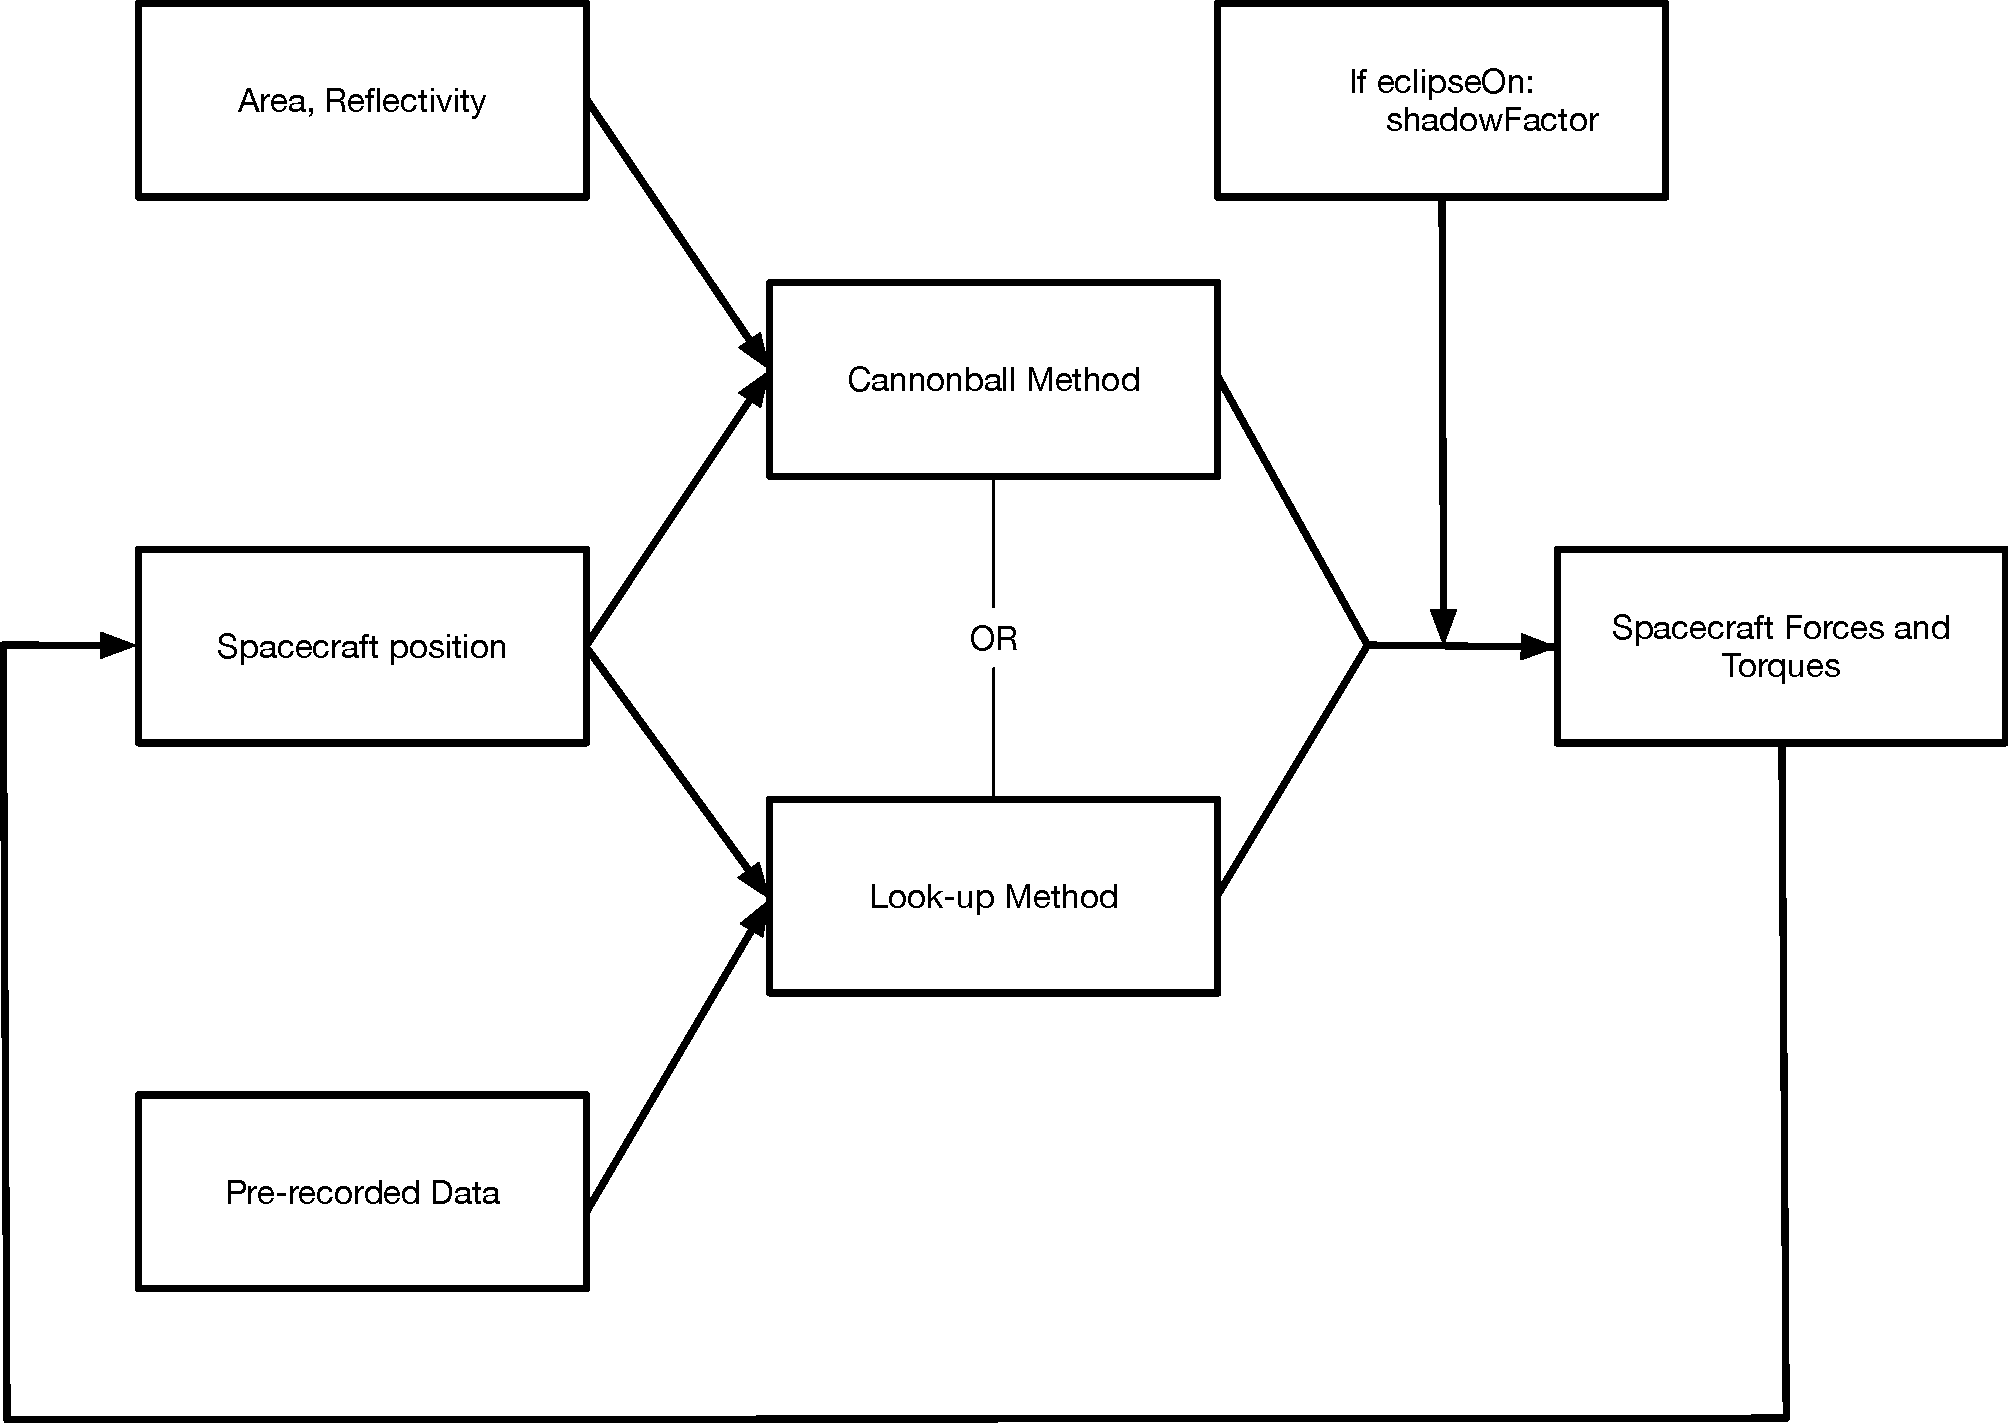
\includegraphics[height=0.6\textwidth, keepaspectratio]{Figures/codeFlow.pdf}
	\caption{A pseudo-code diagram showing the flow of inputs and outputs in the radiation pressure module.}
	\label{img:codeFlow}
\end{figure}

The diagram in Fig. \ref{img:codeFlow} demonstrates the basic iterative logic of the gravity effector module. There is extensive additional code that deals with things from the messaging system to transforming the spacecraft position from one frame to another.

After the inputs are given, radiation\_pressure.cpp calculates the effects of radiation pressure via one of the two methods. At the end, the eclipse factor scales the output forces and torques.
